\documentclass[frenchb,twoside]{EPURapport}

%\usepackage{listings}

%\renewcommand{\lstlistlistingname}{Liste des codes}
%\renewcommand{\lstlistingname}{Code}

%\addextratables{%
%	\lstlistoflistings
%}

%\swapAuthorsAndSupervisors

\RequirePackage{listings}

% le compteur de references
\makeatletter
\newcounter{reference}%
\renewcommand \thereference
 {\@arabic\c@reference}
\makeatother

\newenvironment{bibliographie}{\begin{small}\begin{enumerate}}{\end{enumerate}\end{small}}


\newcommand{\biblioentry}[2]{%
	\refstepcounter{reference}
	\label{#1}
	\ifthenelse{\equal{#2}{}}{%	
		\item[{[\ref{#1}]}] \xspace
	}{%
		\item[{[#2]}] \xspace
	}
}

\newcommand{\biblioentryFull}[5]{%
	\refstepcounter{reference}
	\label{#1}
	\ifthenelse{\equal{#2}{}}{%	
		\item[{[\ref{#1}]}] \xspace #3, \og \textit{#4} \fg, \url{#5}
	}{%
		\ifthenelse{\equal{#5}{}}{%	
			\item[{[#2]}] \xspace \xspace #3, \og \textit{#4} \fg
		}{%
			\item[{[#2]}] \xspace \xspace #3, \og \textit{#4} \fg, \url{#5}
		}
	}
}

\newcommand{\refMot}[1]{%
	\up{[\ref{#1}]}
}

\newcommand{\labelMot}[1]{%
	\refstepcounter{reference}
	\label{#1}
}


\newcommand{\lstinputlistingSmall}[1]{%
	\begin{scriptsize}
		\lstinputlisting{#1}
	\end{scriptsize}
}



%\usepackage[utf8]{inputenc}
\usepackage[utf8x]{inputenc}
\usepackage{ucs}
\usepackage{eurosym}
\usepackage{graphicx}
\usepackage{url}
\usepackage{pdfpages}
\usepackage[makeindex]{glossaries}
%\usepackage{makeidx}
%\usepackage{showidx}

\urlstyle{sf}



%%%%%%%%%%%%Commande personnalisée
\newcommand\motClef[1]{\textbf{\gls{#1}}}
\newcommand{\exemple}{\textbf}
\newcommand{\info}{\textbf}


%\makeindex
\makeglossaries
\thedocument{Projet de r\'{e}alit\'{e} virtuelle}{Construction en Kapla}{Construction en Kapla}

\grade{Département Informatique\\ 5\ieme{} année\\ 2010 - 2011}

\authors{%
	\category{Étudiants}{%
		\name{Guillaume Smaha} \mail{guillaume.smaha@etu.univ-tours.fr}
		\name{Pierre Vittet} \mail{pierre.vittet@etu.univ-tours.fr}
	}
	\details{DI5 2010 - 2011}
}

\supervisors{%
	\category{Encadrant}{%
		\name{Sebastien Aupetit} \mail{aupetit@univ-tours.fr}
		\name{Emmanuel Néron} \mail{emmanuel.neron@univ-tours.fr}
	}
	\details{Université François-Rabelais, Tours}
}

\abstracts{Ce rapport présentera notre projet de logiciel 3D de construction de
Kapla. L'objectif de ce projet était de développer une simulation physique d'un
jeu de Kapla. Nous y expliquerons les différentes techniques utilisées
(signaux, déplacements, ...) pour obtenir le résultat le plus réaliste
possible.}
{Ogre3D, Bullet, Kapla, simulation}
{This report will describe our project of a 3D software for building with
Kapla. The main goal of this project was to develop a physic simulation of a
Kapla game. We will describe the different techniques (signals, movement, …)
used to obtain the most realistic result.}
{Ogre3D, Bullet, Kapla, simulation}


\begin{document}


\chapter{Introduction}

\section{Présentation du projet}
\section{Objectifs}
    L'objectif du projet est de proposer un environnement 3D dans lequel un
    utilisateur peut positionner un ensemble de briquettes afin de créer des
    structures. A partir d'une table, l'utilisateur doit essayer d'obtenir une
    structure qui est la flèche la plus grande possible (c'est à dire qui soit
    éloigné autant que possible du bord de la table.
    Bien sur, chaque briquette est soumis à la force de gravité rendant plus
    complexe l'élaboration de structures stables.
    Ce document décrit les technologies utilisé ainsi que le fonctionnement du
    logiciel.
    \begin{figure}[h]
		\centering
        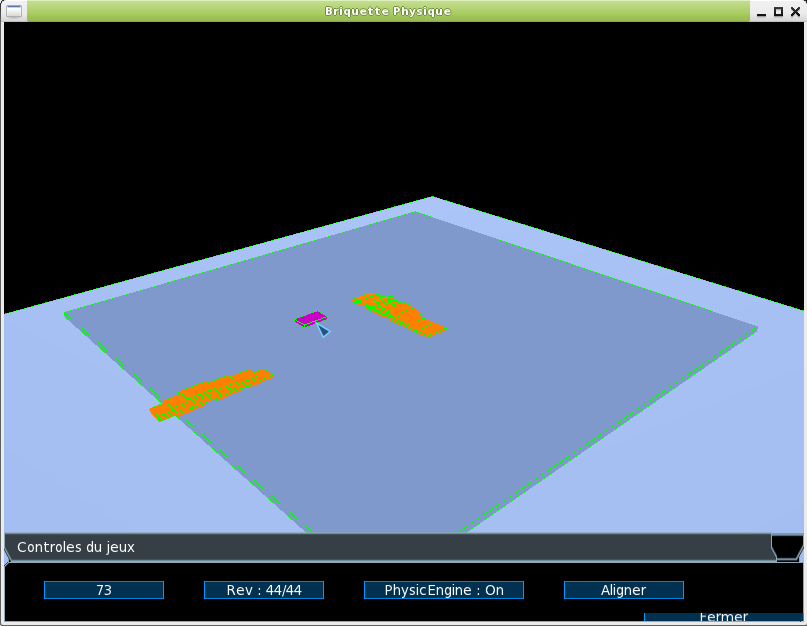
\includegraphics[scale=0.75]{images/jeux.png}
        \caption{\label{fig:jeux}Un exemple typique de l'application en cours de fonctionnment}
    \end{figure}

\section{Détail des attentes}
    Aprés avoir discuter avec notre encadrant, nous nous sommes données les objectifs suivants:
    \begin{itemize}
        \item Un menus permettant de gérer différents niveaux de difficulté.
        Dans un premier temps la seul différence viendra du nombre de
        briquettes disponibles, mais il est également possible de travailler
        sur le poid ou la taille des briquettes.
        \item Saisis des objets et déplacement des briquettes via la souris
        \item Possibilité de revenir à un état précédant ou sucesseur du jeu:
        Aprés chaque placement de briquette, l'état du jeu est mémorisé et on
        permet d'y revenir.
        \item Les briquettes ne doivent pas pouvoir être posés n'importe ou
        mais seulement le long d'un axe. De même, leur orientation est
        vérouillé, l'utilisateur ne pouvant pas placer ces briquettes en
        travers. Cela permet de réduire la complexité du problème lorsque l'on
        recherche des solutions efficaces au problème.
        Le jeu n'est donc en réalité pas un jeu 3D mais 2D, seul la visualisation est en 3D.
        
    \end{itemize}
     \begin{figure}[h]
		\centering
        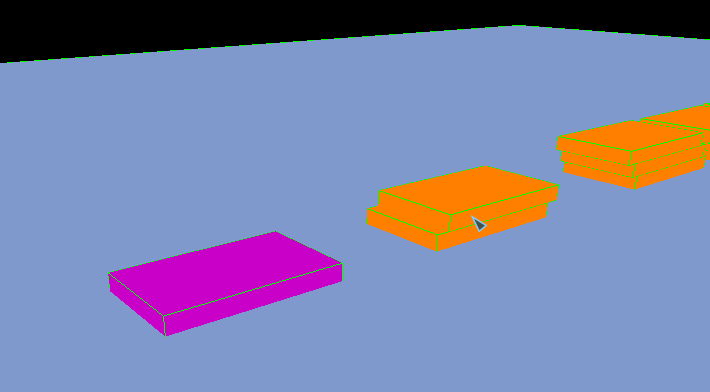
\includegraphics[scale=0.75]{images/zoom_briquette.png}
        \caption{\label{fig:zoom_briquette}Les briquettes sont toutes orientés de la même façon suivant le même axe.}
    \end{figure}

   
    
    
\chapter{Choix techniques}
    \section{Contexte}
    L'encadrant de projet nous à laissé libre de choisir les technologies et
    les outils que l'on souhaitait utilisé pour le projet. Nos choix techniques
    ont été pris de manière à offrir un logiciel facilement utilisable sur
    différentes plateformes mais également en vue d'aller aussi loins que
    possible dans le projet en considérant le temps imparti. Nous avons fait le
    choix de réutiliser autant que possible les outils que nous connaissions
    déja. Cela nous à permis d'avoir une vue d'ensemble et une maitrise que
    nous n'aurions pas eu autrement.

    \section{Liste des outils}
    \begin{itemize}
        \item Ogre\refMot{bib:librairie_ogre}: Moteur 3D open source
        (http://www.ogre3d.org/) supportant aussi bien OpenGL que Direct3D. 
        \item CEGUI\refMot{bib:librairie_cegui}: Crazy Eddie's GUI System
        (http://www.cegui.org.uk) fournissant des outils de créations de menus
        et de fenetre dans un environnement 3D.
        \item Bullet\refMot{bib:librairie_bullet}: Librairie de simulation de
        la physique http://bulletphysics.org/
    \end{itemize}

\chapter{Réalisation}
    \section{Gestion des évènements claviers/souris}
        Nous utilisons une classe PlayerControl qui redirige l'ensemble des
        évènements claviers et souris en des évènements logiques. C'est cette
        classe qui permet de lier les touches à des actions, permettant
        d'abstraire la configuration des touches par la suite.

    \section{Gestion de la caméra}
        Dans ce projet, il n'y a pas besoin de fournir de multiples caméras à
        l'utilisateur. Nous avons convenu que la caméra la plus adapté serait
        une caméra capable de pivoter autours de la table. La caméra est
        toujours orienté vers un point central, qui au départ est le centre de
        la table, cela permet d'avoir une orientation correcte, de plus l'axe
        de lacet de la caméra est fixé sur l'axe Z de façon à ce que la table
        soit toujours vue droite. Les rotations se font à l'aide de la souris,
        il est également possible de zoomer à l'aide des touches du clavier
         ou de la touche centrale de la souris (molette).
        Au départ, nous avons permis avec les touches directionnelles du clavier de
        déplacer le point central qui sert de repère à la caméra, en pratique
        ce n'est pas très utile car peu maîtrisable pour l'utilisateur. Par
        contre, un système beaucoup plus intéresant consiste à déplacer ce point
        central à la position d'une briquette en effectuant un clic droit sur
        celle-ci. La caméra se tourne alors vers la position de la briquette et les rotations
        se font autour de celle-ci.

    \begin{figure}[h]
		\centering
        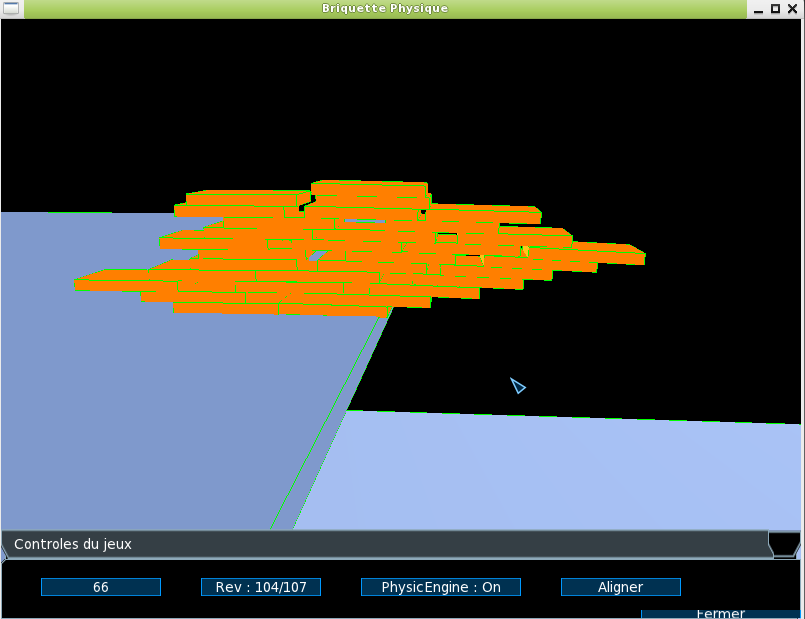
\includegraphics[scale=0.75]{images/bon_score.png}
        \caption{\label{fig:bon_score}Ici l'on voit que la caméra n'est plus centré autours du point
        central de la table mais sur une des briquettes de la structure,
        permettant d'étudier plus précisément celle-ci.}
    \end{figure}

    \section{Gestion de la physique des briquettes}
        La physique est géré avec la librairie Bullet. La technique consite à
        lier à l'objet d'Ogre, un 'corps' particulier à bullet sur lequel
        s'exerceront des forces et sur lequel on surveillera les possibles
        collisions. Bullet permet de rajouter une force d'attraction globale au
        monde et un poid à chacun des objets. Une des difficultés était de
        pouvoir outre-passer la gestion de la physique offerte par bullet lors
        de la sélection des briquettes pour les replacer. Pour cela il a faut
        désactiver l'ensemble des forces s'exercant sur l'objet, permettre les
        deplacements de l'objet (lorsqu'un objet est stable, et qu'il n'y a pas
        de risque que celui ci subisse de nouvelle collision, bullet le bloque
        de façon à ne pas avoir à contrôler continuellement son état), et enfin
        empécher la mise à jour de l'objet et l'application des nouvelles
        forces avant que l'utilisateur n'est fini de positionner l'objet. 

        On utilise en réalité Bullet via OgreBullet pour l'intégrer avec Ogre,
        cependant OgreBullet est limité dans ces possiblités et il nous a
        parfois fallut travailler directement sur l'objet Bullet pour pouvoir
        obtenir le comportement souhaité. 

    \section{Sélection des briquettes}
        Pour sélectionner nos briquettes nous fournissons à l'utilisateur un
        curseur de souris. Lors du clic, un rayon est émis dans la direction de
        celui-ci et qui rapporte l'identifiant d'une briquette éventuellement
        atteinte. C'est également la librairie Bullet qui nous fournis les
        primitives nécessaires. Lorsqu'une briquette est sélectionné, celle-ci
        prend une couleur violette pour avertir l'utilisateur.
        
    \section{Déplacement d'un briquette}
        Pour le déplacement d'une briquette, nous avons tout d'abord voulu
         utiliser la distance parcourue par la souris sur l'écran
        , puis de directement déplacer la briquette en fonction de cette distance en X et Y.
        Le problème est que selon l'orientation de la caméra, la distance en X
        peut s'inverser et donc un déplacement de la souris vers la droit
        déplacerait la briquette vers la gauche.
        
        \
        
        Nous avons donc utilisé une autre méthode.
        Lors de la saisi d'une briquette, on crée un plan sur l'axe de positionnement
        des briquettes, puis nous effectuons un lancer de rayon depuis la position de
        la souris à l'écran. Ce plan possède la même largeur que celle d'une briquette.
        Le plan doit absolument être détruit après le lancer de rayon, sinon celui-ci intérargira avec
        les briquettes comme s'il y avait une collision, et les briquettes seraient alors projeté en dehors
        de leur axe commun Y.
        Lors du déplacement de la souris, le rayon lancé percute alors un point du plan
        , il nous suffit alors de récupérer ce point et de déplacer la briquette aux mêmes
        coordonnées en X et Z que le point de collision (Y étant l'axe commun à toutes les briquettes).
        C'est pour cela, que le centre de la face latérale de la briquette est toujours
		situé à la même position que la souris.
		Deplus le plan ayant une taille limité, il limite alors le déplacement de la briquette dans la scène.
		
		\begin{figure}[h]
			\centering
			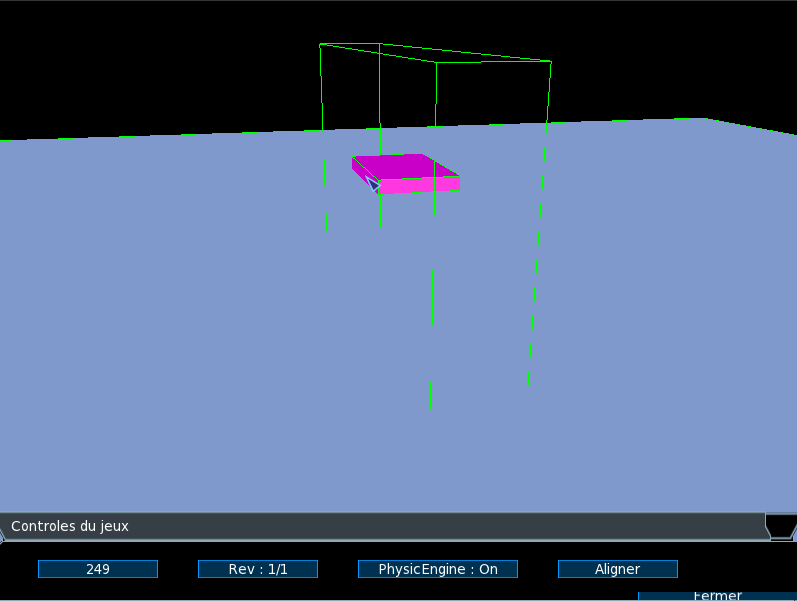
\includegraphics[scale=0.75]{images/move_briquette.png}
			\caption{\label{fig:move_briquette}On peut voir explicitement sur cette image le plan de collision
			qui est nécessaire au déplacement de la briquette.}
		\end{figure}

    \section{Menus}
        Le menus à été réalisé en utilisant la bibliothèque CEGUI. Une classe
        virtuelle Fenetre à été utilisé pour permettre de créer différents
        types de Fenetre. Elle permet en particulier de mettre en place des
        mécanismes en gardant la même apparence graphique pour les différentes
        fenêtres que l'on crée, en offrant des méthodes pour les créer
        simplements. Il suffit d'insérer les boutons ou les éléments graphiques
        sur une fenetre créé automatiquement.
        La charte graphique provient de deux "skins" CEGUI pré-existants et
        placé sous licence libre. Il s'agit de "TaharezLook" qui est le thème
        par défaut de CEGUI et le thème "Sleekspace" que l'on peut télécharger
        sur le site. Ce thème est élégant mais n'est ni complet ni à jour. Je
        l'ai légèrement modifié pour le faire fonctionner (par exemple les
        labels n'apparaissaient plus correctement). Les thèmes utilisent un
        document xml pour décrire le apparence qui est appelé le "Falagard
        looknfell system". J'ai donc travailler dans le fichier xml présent
        dans media/CEGUI/looknfeel/TaharezLook.looknfeel.
        Le logiciel dispose d'un menus d'introdution, simple qui permet de
        choisir le niveau de difficulté via 3 boutons: facile, intérmédiaire,
        difficile.
		\begin{figure}[h]
			\centering
			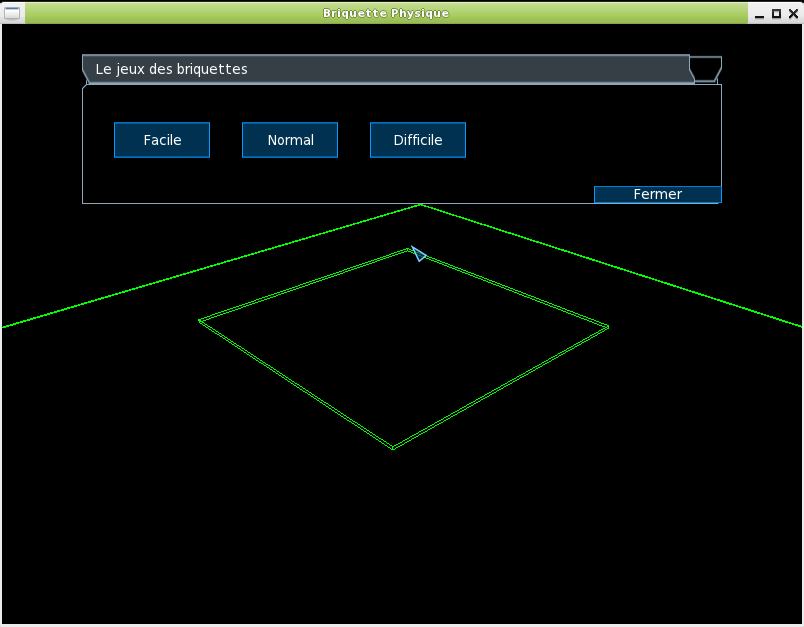
\includegraphics[scale=0.75]{images/Menus_initial.png}
			\caption{\label{fig:menus_initial}Le menus d'introduction au jeu}
		\end{figure}
		\begin{figure}[h]
			\centering
			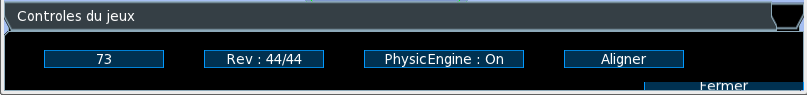
\includegraphics[scale=0.75]{images/menu_jeu.png}
			\caption{\label{fig:menu_jeu}Le menus en cours de jeu}
		\end{figure}      
        Pendant le jeux, un menus est disponible en bas de l'écran. Il est
        également très simple. Il dispose de 4 boutons, le premier affiche le
        nombre de briquettes dont l'utilisateur peut disposé (qui ne sont pas
        encore en jeu). Un clic sur ce bouton permet de faire apparaître une
        briquette sur le plateau de jeu. Le second bouton permet de suivre les
        révision (voir la partie sur les Snapshoots). Celui ci est composé de 2
        numéros, le premier annonce la révision actuelle sur laquelle on se
        trouve, le deuxième, le nombre de révisions accessibles. Les deux
        derniers boutons permettent respectivemnt d'activer ou de désactiver le
        moteur physique et d'aligner les briquettes sur l'axes de construction.

        Au départ, nous avions une souris géré par Ogre (avec un overlay) qui
        permettait à l'utilisateur de viser les briquettes. CEGUI apporte sa
        propre souris. Le plus simple à été de ne conservé visible que la
        souris de CEGUI tout au long du jeu. En pratique, l'on a conservé de
        l'ancienne souris d'ogre qu'un jeu de coordonnées mis à jour à chaque
        déplacement de la souris de CEGUI afin de garder la synchronisation
        entre les deux.
\chapter{Conclusion}




\chapter{Bibliographie}

\begin{bibliographie}	
	\biblioentry{bib:ogre_quaternion}{} Ogre Wiki, \textit{Utilisation des quaternions dans Ogre}, \url{http://www.ogre3d.org/tikiwiki/Quaternion+and+Rotation+Primer}
	\biblioentry{bib:librairie_ogre}{} Ogre Documentation, \textit{Documentation Doxygen d'Ogre}, \url{http://www.ogre3d.org/docs/api/html/index.html}
	\biblioentry{bib:librairie_cegui}{} CEGUI Wiki, \textit{Utilisation de CEGUI}, \url{http://www.cegui.org.uk/wiki/index.php/Main_Page}
	\biblioentry{bib:librairie_bullet}{} Bullet Wiki, \textit{Utilisation de Bullet}, \url{http://bulletphysics.org/wordpress/}
	\biblioentry{bib:librairie_ogrebullet}{} Ogre Wiki, \textit{Tutorial d'utilisation d'OgreBullet}, \url{http://www.ogre3d.org/tikiwiki/OgreBullet}
	\biblioentry{bib:signaux_qt}{} Site du Zéro, \textit{Signaux avec QT}, \url{http://www.siteduzero.com/tutoriel-3-11268-les-signaux-et-les-slots.html}
	\end{bibliographie}	


\end{document}
